\chapter{The Collatz Tree}

\section{The Connection between Groups and Graphs}
\label{sec:groups_graphs}
Let $(a_k)$ be a numerical sequence with $a_k=g^{(k)}(m)$, then a reversion produces an infinite number of sequences of reversely-written Collatz members \cite{Ref_Klisse_2010}.

\par\medskip
Let $S$ be a set containing two elements $q$ and $r$, which are bijective 
functions over $\mathbb{Q}$:
\begin{equation}
\begin{array}{l}
q(x)=2x \\ 
r(x)=\frac{1}{3}(x-1)
\end{array}
\end{equation}

Let a binary operation be the right-to-left composition of functions
$q\circ r$, where $q\circ r(x)=q(r(x))$. Composing functions is an
associative operation. All compositions of the bijections $q$ and $r$
and their inverses $q^{-1}$ and $r^{-1}$ are again bijective. The set,
whose elements are all these compositions, is closed under that operation.
It forms a free group $F$ of rank 2 with respect to the free generating set $S$, where the group's binary operation $\circ$ is the function composition and the group's identity element is the identity function $id_{\mathbb{Q}}=e$. We call $e$ an \textit{empty string}. $F$ consists of all expressions (strings) that can be concatenated from the generators $q$ and $r$. The corresponding Cayley graph $Cay(F,S)=G$ is a regular tree whose vertices have four neighbors \cite[p.~66]{Ref_Loeh}. A tree is called \textit{regular} or \textit{homogeneous} when every vertex has the same degree, in this case, $d(v)=4$ for every vertex $v$ in $G$. The Cayley graph's set of vertices is $V(G)=F$, and its set of edges is $E(G)=\left\{\left\{f,f\circ s\right\}\mid f\in F,s\in\left(S\cup S^{-1}\right)\setminus\left\{e\right\}\right\}$ \cite[p.~57]{Ref_Loeh}. More precisely, the vertices are \textit{labeled} by the elements (strings) of $F$.

\par\medskip
In conformance with graph-theoretical precepts \cite{Ref_Bondy_Murty},
\cite{Ref_Bonnington_Little}, \cite{Ref_Bender_Williamson}
we specify a subgraph $H$ of $G$ as a triple
$\left(V(H),E(H),\psi_{H}\right)$ consisting of a set $V(H)$ of vertices,
a set $E(H)$ of edges, and an incidence function $\psi_{H}$. The latter
is, in our case, the restriction $\psi_{G}\vert_{E(H)}$ of the Cayley
graph's incidence function to the set of edges that only join vertices,
which are labeled by a string over alphabet $\{r,q\}$ without the inverses:
$E(H)=\left\{\left\{f,f\circ s\right\}\mid f\in F,s\in S\setminus\left\{e
\right\}\right\}$.

\par\medskip
This subgraph corresponds to the monoid $S^*$, which is freely generated
by $S$ follows related thoughts \cite{Ref_Truemper_2014} that examine
the Collatz problem in terms of a free semigroup on the set $S^{-1}$ of
inverse generators. Note that this semigroup is not to be confused with an
\textit{inverse semigroup} "in which every element has a unique inverse"
\cite[p.~26]{Ref_Almeida}, \cite[p.~22]{Ref_Loeh}.

\par\medskip
Let $Y^X=\{f\mid f\text{ is a map }X\rightarrow Y\}$ be the set of functions, which in category theory is referred to as the \textit{exponential object} for any sets $X$, $Y$. The evaluation function $ev:Y^X\times X\to Y$ sends the pair $(f,x)$ to $f(x)$. For a detailed description of this concept, see \cite[p.~127]{Ref_Johnsonbaugh}, \cite[p.~155]{Ref_MacLane_Birkhoff}, \cite[p.~54]{Ref_Novak_etal} and \cite[p.~188]{Ref_Pellissier}. We define the evaluation function $ev_{S^*}:S^*\times\{1\}\rightarrow\mathbb{Q}$ that evaluates an element of $S^*$, id est a composition of $q$ and $r$, for the given input value $1$. Furthermore we define the corestriction ${ev^0_{S^*}}$ of $ev_{S^*}$ to $\mathbb{N}$. Since a corestricion of a function resricts the function's codomain \cite[p.~3]{Ref_Helemskii}, the function $ev^0_{S^*}$ operates on a subset $T\subset S^*$ that contains only those compositions of $q$ and $r$, which return a natural number when inputting the value $1$.

\par\medskip
The set $T$ forms not a monoid under function composition, for example $ev_{S^*}(qrq^4,1)=10$ and $ev_{S^*}(rq^6,1)=21$, but the composition $qrq^4rq^6$ does not lie in $T$, because the evaluation $ev_{S^*}(qrq^4rq^6,1)$ yields a value outside the codomain $\mathbb{N}$. However, each element of this set labels a vertex of a tree $H_{T}\subset H$, which is a proper subtree of $H$.

\par\medskip
Let $U\subset T$ be a subset of $T$, which does not contain a reduced word with two or more successive characters $r$. The corresponding tree $H_{U}\subset H_{T}$ reflects Collatz sequences as demonstrated in figure~\ref{fig:1}.

\begin{remark}
When talking about trees having a root ("rooted trees"), another important concept should be explained: the \textbf{level of a vertex} or often called \textbf{depth of a vertex} is the length of the path from the root to this vertex \cite[p.~804]{Ref_Rosen}. In other words, it is the vertex's distance (the number of edges in the path) from the root. The \textbf{height of a vertex} is its level plus one $level(v)+1=height(v)$, see \cite[p.~169]{Ref_Makinson}.
\end{remark}

% trim=left top right bottom
\begin{figure}
	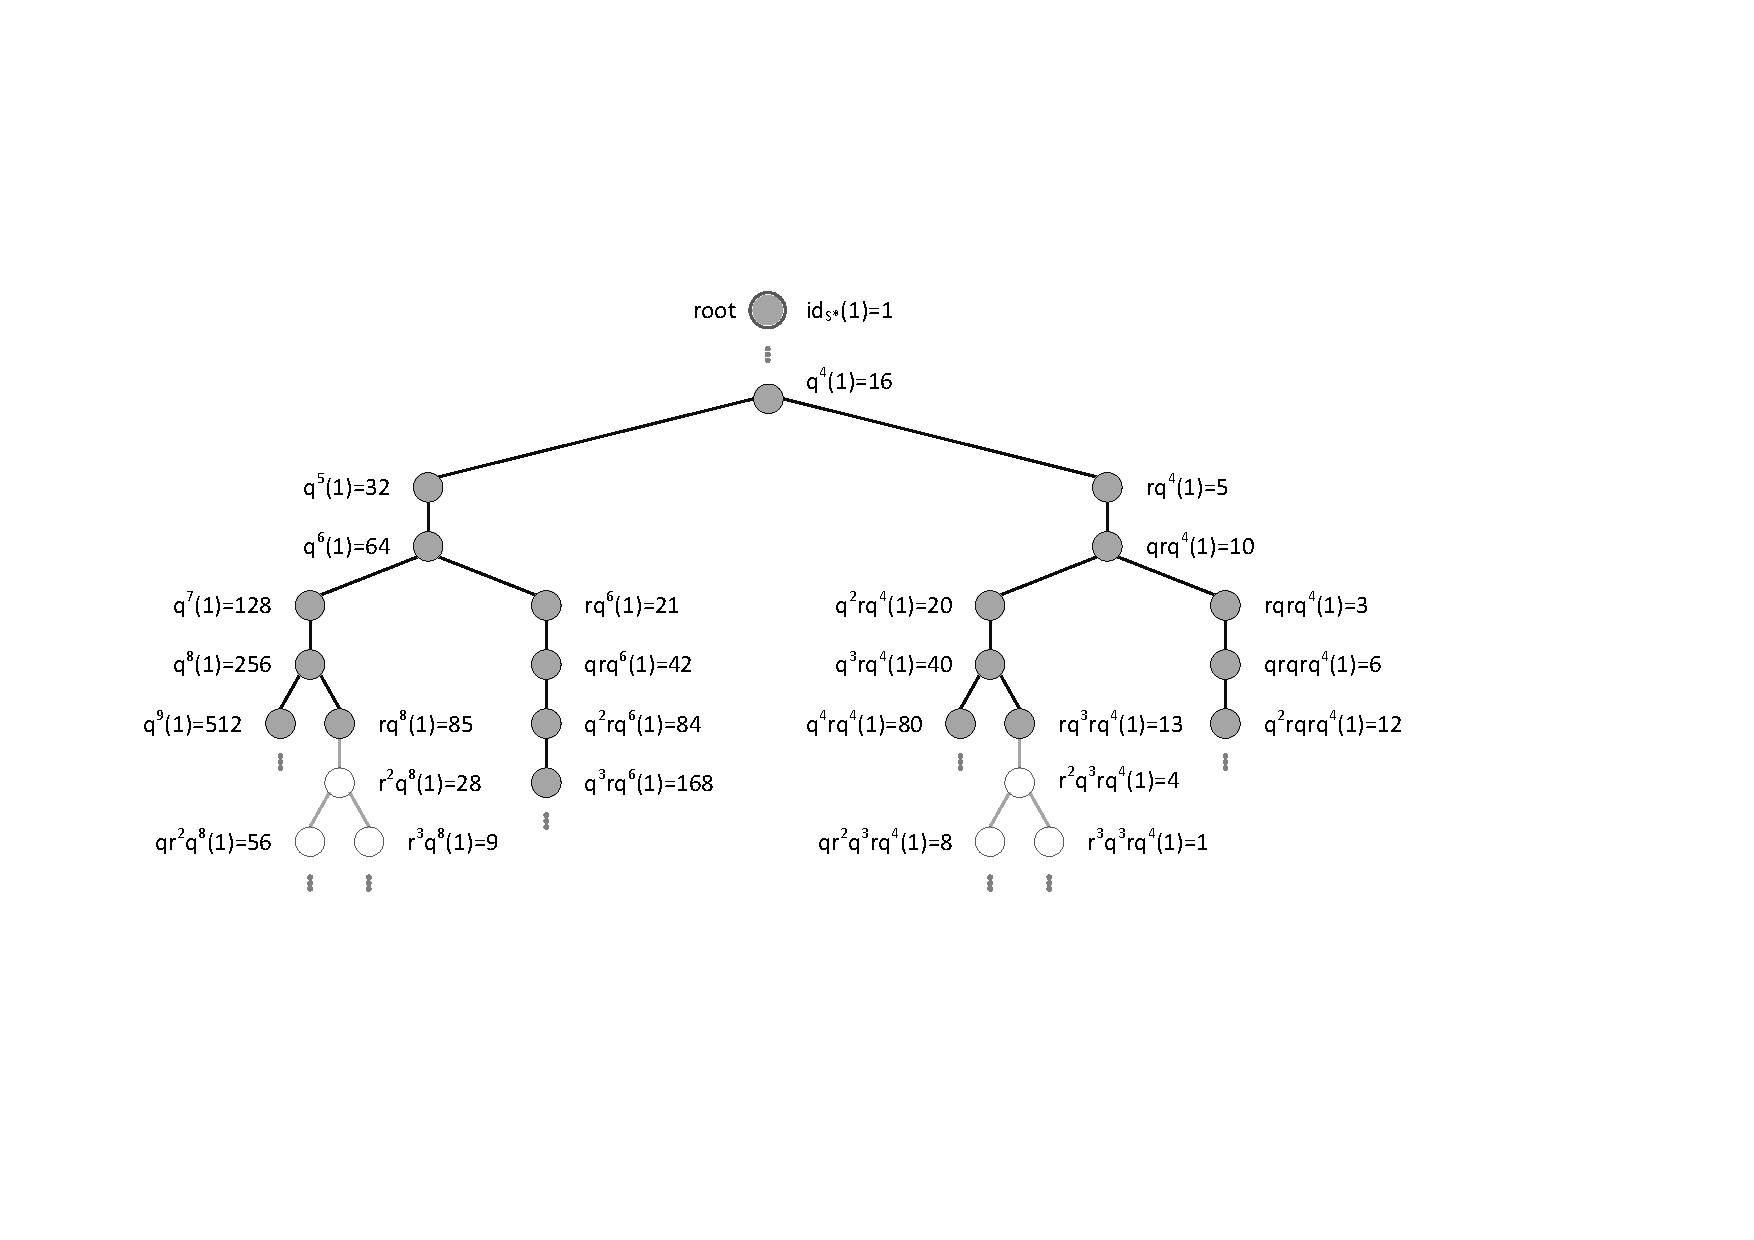
\includegraphics[trim=2.3cm 5.8cm 5.9cm 4.8cm, 
	width=1.00\textwidth,page=1]{figures/caytree.pdf}
	\caption{Small section of $H_T$ with darkly highlighted subtree $H_U$}
	\label{fig:1}
\end{figure}

\section{Defining the Tree}
The starting point for specifying our tree is $H_U$. Due to its
significance, we first concertize $H_U$ by the definition~\ref{def:H_U}
below, which establishes four essential characteristics.

\pagebreak
\begin{definition}
The graph $H_U$ possess the following key properties:
\begin{itemize}
	\item \mbox{\boldmath$H_U$} \textbf{is a directed graph (digraph):} Fundamentally, when we consider the more general case, an undirected graph as a triple $(V,E,\psi)$, the incidence function maps an edge to an arbitary vertex pair $\psi : E\rightarrow\{X\subseteq V:\left|X\right|=2\}$. In a digraph, the set $V\times V$ represents ordered vertex pairs. Accordingly the incidence function is more specifically defined, namely as a mapping of the edges to that set $\psi : E\rightarrow\{(v,w)\in V\times V:v\neq w\}$, see \cite[p.~15]{Ref_Korte_Vygen}.
	\item \mbox{\boldmath$H_U$} \textbf{is a rooted tree:} According to Rosen \cite[p.~747]{Ref_Rosen}, a rooted tree is "a tree in which one vertex has been designated as the root and every edge is directed away from the root." Peculiarly, this definition considers the directionality as an inherent part of rooted trees. Unlike Mehlhorn and Sanders \cite[p.~52]{Ref_Mehlhorn_Sanders}, for example, who distinguish between an undirected and directed rooted tree.
	\par\smallskip
	\textit{Note: As long as we do not stipulate that vertices may collapse, it is absolutely guaranteed that the graph is a tree.}
	\item \mbox{\boldmath$H_U$} \textbf{is an out-tree:} There is exactly one	path from the root to every other node \cite[p.~52]{Ref_Mehlhorn_Sanders}, which means that edge directions go from parents to children \cite[p.~108]{Ref_Du_Ko_Hu}. This property is implied in Rosen's definition for a rooted tree as well by saying "every edge is directed away from the root." An out-tree is sometimes designated as \textit{out-arborescence} \cite[p.~108]{Ref_Du_Ko_Hu}.
	\item \mbox{\boldmath$H_U$} \textbf{is a labeled tree:} For defining a labeled graph, Ehrig et al. \cite[p.~23]{Ref_Ehrig_etal} use a label alphabet consisting of a vertex label set and an edge label set. Since we only label the vertices, in our case the specification of a vertex label set $L_V$ together with the vertex label function $l_V:V\rightarrow L_V$ is sufficient. Originally, we said vertex labels are strings over the alphabet $S=\{q,r\}$, through which the free monoid $S^*$ is generated. We illustrate labeling $H_U$ by defining $l_{V(H_U)}(v)=ev^0_{S^*}(l_{V(G)}(\iota(v)),1)$, whereby $\iota:V(H_U)\hookrightarrow V(G)$ is the inclusion map \cite[p.~142]{Ref_Childs} from the set of vertices of $H_U$ to the set of vertices from the previously defined Cayley graph $G$.
\end{itemize}
\label{def:H_U}
\end{definition}

\par\medskip
We define a tree $H_C$ by taking the tree $H_U$ as a basis and for every
vertex $v\in V(H_U)$ satisfying $2\mid l_{V(H_U)}(v)$, we contract the
incoming edge. We attach the label of the parent of $v$ to the new
vertex, which results by replacing (merging) the two overlapping
vertices that the contracted edge used to connect. Visually, we
obtain $H_C$ by contracting all edges in $H_U$ that have an even-labeled 
target vertex, which (due to contraction) gets "merged into its parent." 
Edge contraction is occasionally referred to as \textit{collapsing an 
edge}. For more details and examples on edge contraction, one can see
Voloshin \cite[p.~27]{Ref_Voloshin} and Loehr \cite{Ref_Loehr}.

\par\medskip
The tree $H_C$ is a \textit{minor of $H_U$}, since it can be obtained
from $H_U$ "by a sequence of any vertex deletions, edge deletions and
edge contractions" \cite[p.~32]{Ref_Voloshin}. The sequence of contracting
the edges between adjacent (in our case even-labeled) vertices is called
\textit{path contraction}.

\par\medskip
A small section of the tree $H_C$ is shown in figure~\ref{fig:2}. Other
definitions of the same tree exist, see for example Conrow 
\cite{Ref_Conrow} or Bauer \cite[p.~379]{Ref_Bauer}.

\begin{figure}
	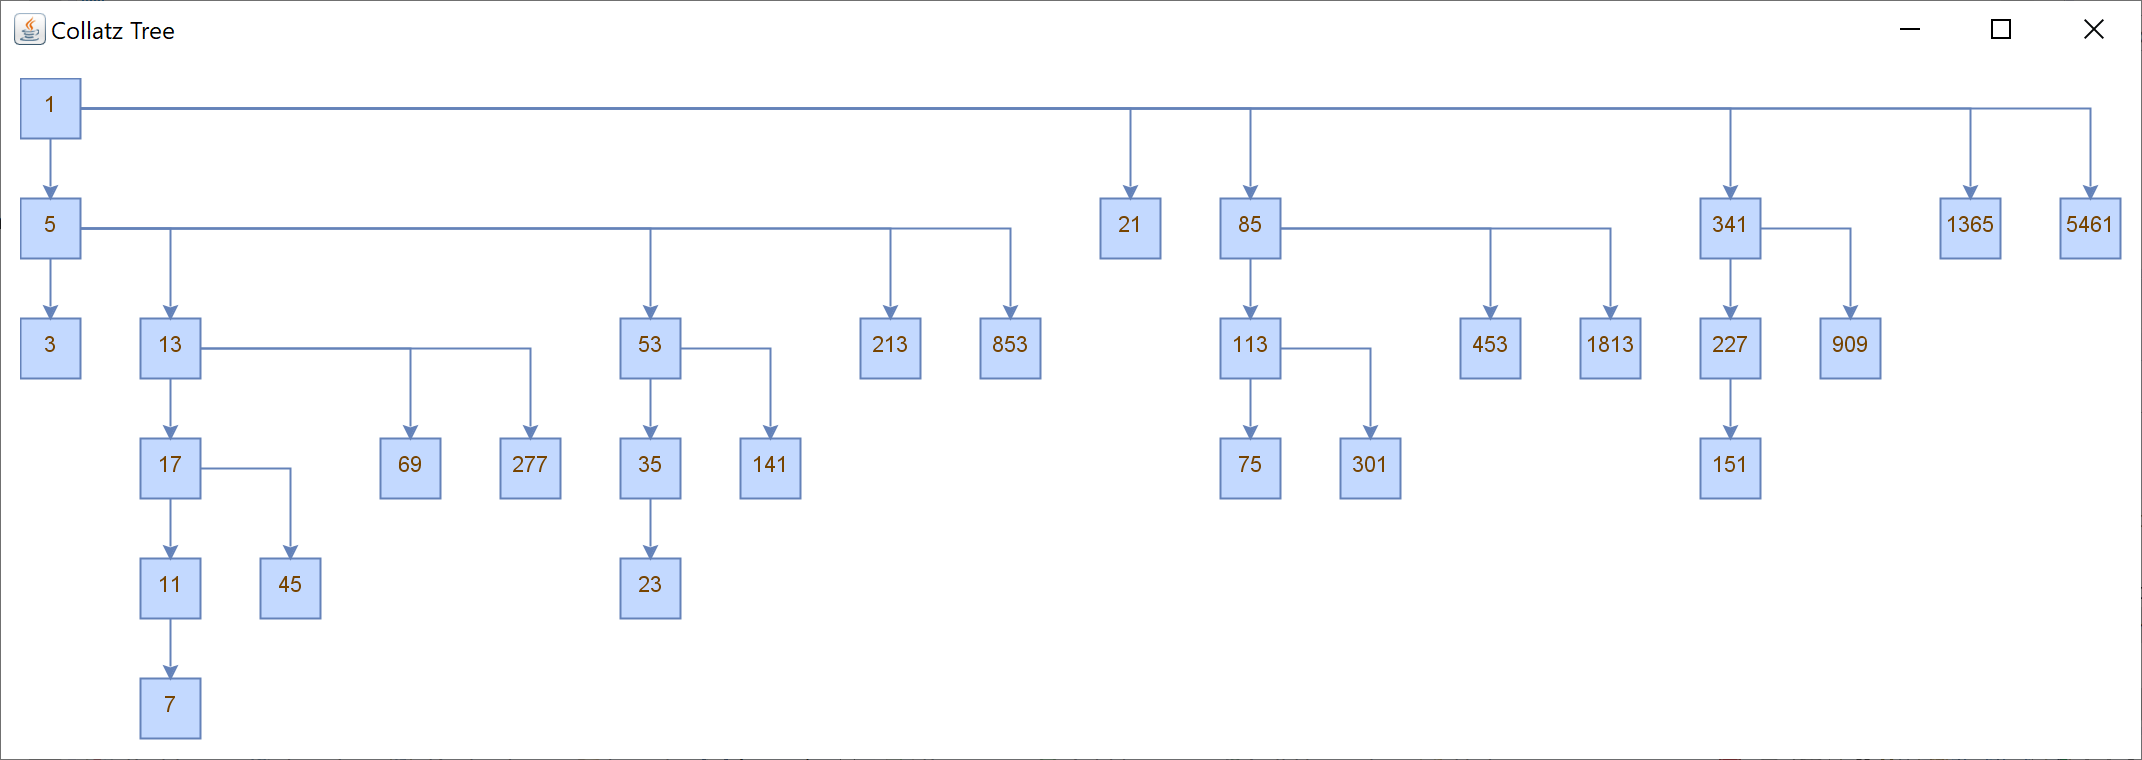
\includegraphics[width=1.00\textwidth]{figures/h_c.png}
	\caption{Small section of $H_C$ (displaying the trivial cycle is waived)}
	\label{fig:2}
\end{figure}

\section{Relationship of successive nodes in \mbox{$H_C$}}

Let $v_1$ and $v_{n+1}$ be two vertices of $H_C$, where $v_1$ is reachable from $v_{n+1}$ with $level(v_1)-level(v_{n+1})=n$. Hence, a path $(v_{n+1},\ldots,v_1)$ exists between these two vertices. Theorem~\ref{theo:1} specifies the following relationship between $v_1$ and $v_{n+1}$.

\par\medskip
\begin{theorem}
	\label{theo:1}
	$l_{V(H_C)}(v_{n+1})=3^nl_{V(H_C)}(v_1)\prod_{i=1}^{n}\left(1+\frac{1}{3l_{V(H_C)}(v_{i})}\right)2^{-\alpha_i}$.
	In order to simplify readability, we waive writing down the vertex label function and put it shortly:\\
	$v_{n+1}=3^nv_1\prod_{i=1}^{n}\left(1+\frac{1}{3v_{i}}\right)2^{-\alpha_i}$.
	The value $\alpha_i\in\mathbb{N}$ is the number of edges which have been contracted between $v_i$ and $v_{i+1}$ in $H_U$.
\end{theorem}

In order to demonstrate the construction produced by theorem~\ref{theo:1} in an illustrative fashion, example~\ref{ex:vertices} runs through a concrete path in $H_C$.

\par\medskip
\begin{example}
	\label{ex:vertices}
	For example, the two vertices $v_1=45$ and $v_{1+3}=v_4=5$ are 
	connected
	via the path $(5,13,17,45)$, see figure~\ref{fig:2}. Furthermore, one
	can retrace in figure~\ref{fig:3} the uncontracted path between these
	two nodes within $H_U$. When applied to this example,
	theorem~\ref{theo:1} produces the following:	
	\begin{center}
		$5=v_{1+3}=3^3*45*\left(1+\frac{1}{3*45}\right)*2^{-3}
		*\left(1+\frac{1}{3*17}\right)*2^{-2}
		*\left(1+\frac{1}{3*13}\right)*2^{-3}$
	\end{center} 
\end{example}
\begin{proof}
	\label{proof:1}
	This relationship of successive nodes can simply be proven inductively. For the base case, we set $n=1$ and retrieve
	\begin{center}
		$v_{1+1}=3v_1\left(1+\frac{1}{3v_1}\right)2^{-\alpha_1}
		=\left(3v_1+1\right)2^{-\alpha_1}=v_2$
	\end{center}
	The path from $v_2$ to $v_1$ can conformly be expressed by a string $rq\cdots q$ of $S^*$, because of $v_1=r\circ q^{\alpha_1}\left(v_2\right)$. We set $n=n+1$ for the step case, which leads to
	\begin{equation*}
	\begin{array}{cl}
	v_{n+2} &
	=3^{n+1}v_1\prod_{i=1}^{n+1}\left(1+\frac{1}{3v_i}\right)2^{-\alpha_i}\\
	&
	=3^{n+1}v_1\left(1+\frac{1}{3v_{n+1}}\right)2^{-\alpha_{n+1}}\prod_{i=1}^{n}\left(1+\frac{1}{3v_i}\right)2^{-\alpha_i}\\
	&
	=3\left(1+\frac{1}{3v_{n+1}}\right)2^{-\alpha_{n+1}}3^nv_1\prod_{i=1}^{n}\left(1+\frac{1}{3v_i}\right)2^{-\alpha_i}\\
	&
	=3\left(1+\frac{1}{3v_{n+1}}\right)2^{-\alpha_{n+1}}v_{n+1}\\
	&
	=\left(3v_{n+1}+1\right)2^{-\alpha_{n+1}}
	\end{array}
	\end{equation*}
	In this case the path from $v_{n+2}$ to $v_{n+1}$ is conformly 
	expressable by a string $rq\cdots q$ of $S^*$ too, since
	$v_{n+1}=r\circ q^{\alpha_{n+1}}\left(v_{n+2}\right)$.
\end{proof}

Even though the tree may theoretically contain two or more identically labeled vertices, it is essential to emphasize that we only consider such paths $(v_{n+1},\ldots,v_1)$ whose vertices are all labeled differently. Later in section~\ref{sec:cycles}, we even require that identically labeled nodes are one and the same. In order to correctly determine successive nodes using theorem~\ref{theo:1}, we must consider the halting conditions. These are specified in Definition~\ref{def:halting_condition}.

\begin{definition}
	\label{def:halting_condition}
	When determining successive nodes starting at $v_1$ according to theorem~\ref{theo:1}, we halt if one of the following two conditions is fulfilled:
	\begin{enumerate}
		\item $v_{n+1}=1$
		\item $v_{n+1}\in\{v_1,v_2,\ldots,v_n\}$
	\end{enumerate}
	If the first condition applies, the Collatz conjecture is true for a specific sequence. When the second condition is fulfilled, the sequence has led to a cycle. For every starting node, except the root node (labeled with $1$), the Collatz conjecture is consequently falsified. Let us consider the example $v_1=13$, where the algorithm halts after two iterations, because the first condition is met:
	\[
	v_{n+1}=3^2\cdot\left(1+\frac{1}{3\cdot13}\right)\left(1+\frac{1}{3\cdot5}\right)\cdot2^{-7}=1
	\]
	
	If we examine the case $v_{1}=1$, we realize that the algorithm finishes after the first iteration, since both halting conditions are true. The sequence stops because the final node labeled with $1$ is reached. Furthermore, the sequence has led to a cycle:
	\[
	v_{n+1}=3\cdot\left(1+\frac{1}{3}\right)2^{-2}=1
	\]
	
	The trivial cycle is the only sequence where both conditions are fulfilled.
\end{definition}

\noindent
Theorem~\ref{theo:1} can be used for specifying the condition of a cycle as follows:

\begin{equation}
\label{eq:func_cycle}
\begin{array}{l}
v_{1}=3^nv_1\prod_{i=1}^{n}\left(1+\frac{1}{3v_i}\right)2^{-\alpha_i}
\\[\medskipamount]
2^{\alpha_1+\cdots+\alpha_n}=\prod_{i=1}^{n}\left(3+\frac{1}{v_i}\right)
\end{array}
\end{equation}

A similar condition has been formulated by Hercher \cite{Ref_Hercher}. Taking a first look at equation~\ref{eq:func_cycle}, we are able to recognize the trivial cycle for $n=1$. One might easily come to the false conclusion that the term only results in a natural number for this trivial cylce, since we are multiplying fractions. The following counterexample, starting at $v_1=31$, disproves this assumption:
\begin{equation*}
20480=\left(3+\frac{1}{31}\right)\left(3+\frac{1}{47}\right)
\left(3+\frac{1}{71}\right)\left(3+\frac{1}{107}\right)\left(3+\frac{1}{161}\right)\left(3+\frac{1}{121}\right)\left(3+\frac{1}{91}\right)\left(3+\frac{1}{137}\right)\left(3+\frac{1}{103}\right)
\end{equation*}

According to OESIS \cite{Ref_OESIS}, the integer $v_1=31$ is called \textit{self-contained}. The term self-contained is based on the fact that the node $v_{n+1}=v_{10}=155$ is divisible by the starting node $v_1=31$. Moreover, $v_{10}$ results from applying one and the same function (in this case the Collatz function) using $v_1$ as input, see also Guy \cite[p.~332]{Ref_Guy}. For such a case equation~\ref{eq:func_cycle} leads to a natural number, but not necessarily to a cycle. A cycle only occurs if the term results in a power of two. One example is the trivial cycle. We find another case when we choose the factor $5$ instead of $3$:
\begin{center}
	$128=2^7=\left(5+\frac{1}{13}\right)\left(5+\frac{1}{33}\right)
	\left(5+\frac{1}{83}\right)$
\end{center}

The above example shows that non-trivial cycles can be found if we generalize the Collatz conjecture by replacing the factor $3$ with the variable $k$. We study this generalized form and the occurance of cycles in chapter \ref{sec:cycles}. A detailed elaboration of the divisibility and a deeper understanding of the tree $H_C$ needs to be performed in order to get towards any proof of the Collatz conjecture.

%\par\medskip\noindent
%Generally, for any variant $kx+1$ it applies that if $v_1\mid v_{n+1}$, the the product is natural:
%\begin{equation*}
%	\prod_{i=1}^n\left(k+\frac{1}{v_i}\right)\in \mathbb{N}
%\end{equation*}

\begin{figure}
	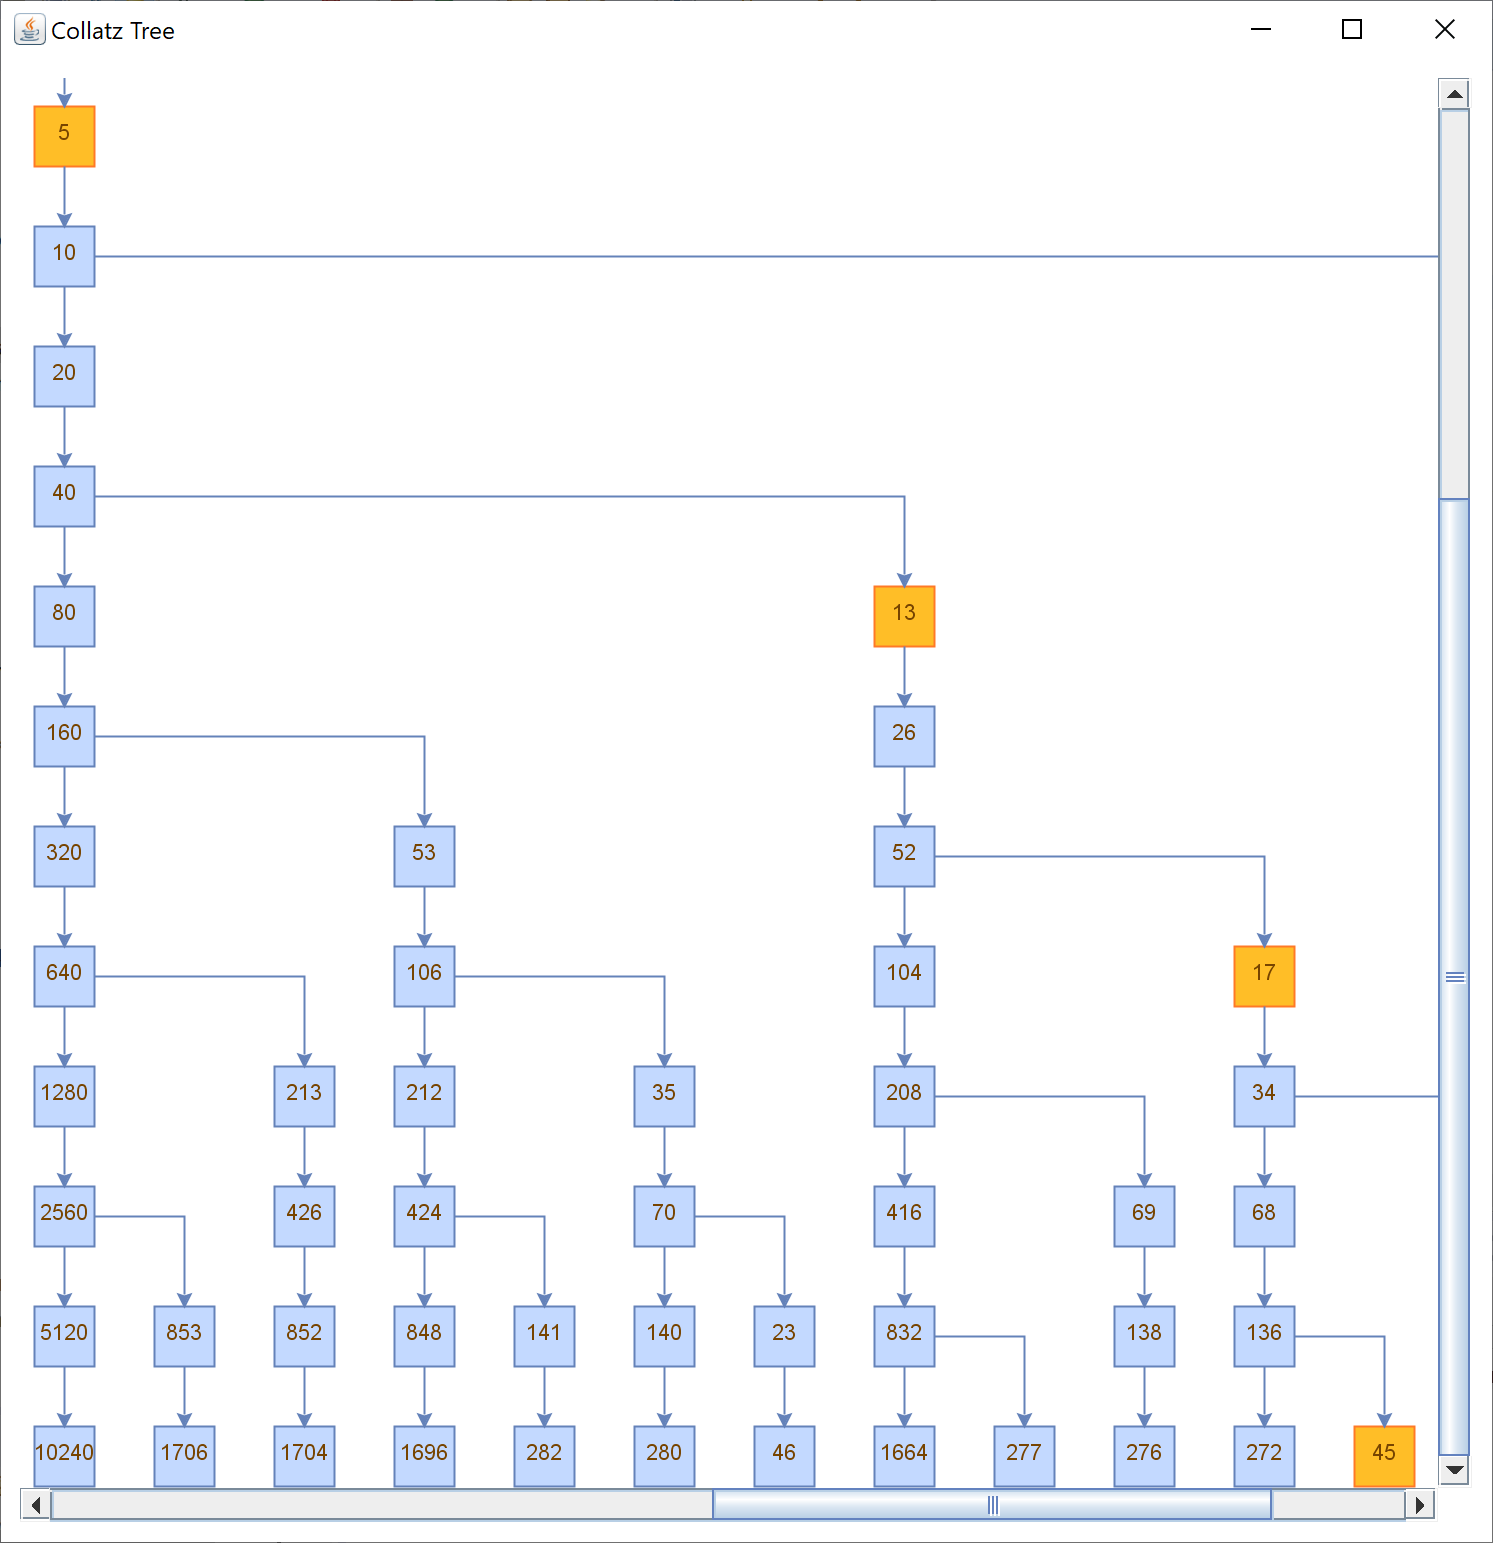
\includegraphics[width=1.00\textwidth]{figures/h_u.png}
	\caption{Section of $H_U$ containing the path from $5$ to $45$}
	\label{fig:3}
\end{figure}

\section{Relationship of sibling nodes in \mbox{$H_C$}}
In a rooted tree, vertices which have the same parent are called "siblings" \cite[p.~702]{Ref_Johnsonbaugh}, \cite[p.~747]{Ref_Rosen}. Sibling vertices accordingly have the same level.

\par\medskip
Let $w$ be a vertex, from which a path exists to the vertex $v_1$. Let $v_2$ be the immediate right-sibling of $v_1$, then $l_{V\left(H_C\right)}\left(v_2\right)=4*l_{V\left(H_C\right)}\left(v_1\right)+1$. This fact has been expressed differently by Kak \cite{Ref_Kak_2014} as follows: "If an odd number $a$ leads to another odd number (after several applications of the Collatz transformation) $b$, then $4a+1$ also leads to $b$."

\par\medskip
Applied to our approach, consider $w$ as the parent of $v_1$ and $v_2$. Suppose, in $H_U$, a path consisting of $n+1$ edges goes from $w$ to $v_1$. Then we can straightforwardly show that $n$ edges in $H_U$ have been contracted between both nodes $w$ and $v_1$ and $n+2$ edges between $w$ and $v_2$ (for simplicity we again omit writing the label function):
\begin{equation*}
\begin{array}{l}
		v_1=\frac{w*2^n-1}{3}
		\\[\medskipamount]
		v_2=\frac{w*2^{n+2}-1}{3}=4*v_1+1
\end{array}
\end{equation*}

For example, $n=3$ edges in $H_U$ have been contracted between $w=5$ and $v_1=13$ and $n+2=5$ edges between $w$ and $v_2=53$, whereby in $H_C$, the vertex $v_2$ is the right-sibling of $v_1$ and these two sibling vertices are immediate children of $w$.

\section{A vertex's \mbox{$n$}-fold left-child and right-sibling in \mbox{$H_C$}}
Referring to the "left-child, right-sibling representation" of rooted trees \cite[p.~246]{Ref_Cormen_Leiserson_Rivest_Stein}, the function $\textit{left-child}:V\rightarrow V$ returns the leftmost child of a vertex $v$. Nesting this function $n$ times leads to the definition of a vertex's $n$-fold left-child, which is given by $\textit{left-child}^n(v)$. As shown in figure~\ref{fig:2}, for example $\textit{left-child}^3(13)=7$.

\par\medskip
The function $\textit{right-sibling}:V\rightarrow V$ points to the sibling of a vertex $v$ immediately to its right \cite[p.~246]{Ref_Cormen_Leiserson_Rivest_Stein}. If this function is nested $n$ times, we get a vertex's $n$-fold right-sibling defined by $\textit{right-sibling}^n(v)$. One example is $\textit{right-sibling}^2(113)=1813$ which has been demonstrated in figure~\ref{fig:2} too.

\par\medskip
Let $w$ be a vertex in $H_C$ and $v_0$ the left-child of $w$. The $n$-fold right-sibling of $v_0$ can be calculated as follows:
\begin{equation}
\label{eq:nfold_right_sibling}
	v_n=\textit{right-sibling}^n(v_0)=\frac{1}{3}*\left(w*2^{2*n+\pi_3(w\bmod 3)}-1\right)
\end{equation}

The function $\pi_3$ is the self-inverse permutation (involution):
\begin{equation}
\label{eq:pi_3}
	\pi_3=\left(\begin{array}{cc}
	1 & 2\\
	2 & 1
	\end{array}\right)
\end{equation}
We consider permutations of the set $\{1,2\}$ and not of $\{0,1,2\}$, due to the fact that $w\bmod 3$ cannot be zero. A node $w$ in $H_C$, which is labeled by an integer divisible by $3$ is a leaf; and therefore such node has no left-child, more specifically it has no children at all.

\par\medskip
\noindent
When setting $n=0$, we trivially retrieve the vertex's $w$ left-child:
\begin{center}
	$v_0=\textit{left-child}(w)=\frac{1}{3}*\left(w*2^{\pi_3(w\bmod 3)}-1\right)$
\end{center}

\begin{example}
	\label{ex:siblings}
	Let us refer to figure~\ref{fig:2} again and pick out $w=5$. Then the
	vertex's $w$ left-child is $v_0=3$ and the threefold right-sibling
	$v_3=213$:

	\begin{equation*}
	\begin{array}{l}
		v_0=\frac{1}{3}*\left(5*2^{\pi_3(5\bmod 3)}-1\right)=3
		\\[\medskipamount]
		v_3=\frac{1}{3}*\left(5*2^{2*3+\pi_3(5\bmod 3)}-1\right)=213
	\end{array}
	\end{equation*}
\end{example}

\section{Left-child and right-sibling in the \mbox{$5x+1$} variant of \mbox{$H_C$}}
In the following we take a look at the $5x+1$ variant of $H_C$. We name this graph $H_{C,5}$ and must note that it is not a tree and moreover that not all of its vertices are reachable from the root. We define the permutation $\pi_5$ as follows:
\begin{center}
	$\pi_5=\left(\begin{array}{cccc}
		1 & 2 & 3 & 4\\
		4 & 3 & 1 & 2
	\end{array}\right)$	
\end{center}

Next, by letting $w$ be a vertex in $H_{C,5}$ and $v_0$ the left-child of $w$
we obtain the $n$-fold right-sibling of $v_0$ by the function that
is slightly different to the one defined by \ref{eq:nfold_right_sibling}:
\begin{equation}
\label{eq:nfold_right_sibling_5}
	v_n=\textit{right-sibling}^n(v_0)=\frac{1}{5}*\left(w*2^{4*n+\pi_5(w\bmod 5)}-1\right)
\end{equation}

Analogous to \ref{eq:pi_3} only permutations on the set without zero
\{1,2,3,4\} need to be considered, since $w\bmod 5$ cannot be zero.
Otherwise, if $w\equiv 0 (\bmod 5)$ which means that $w$ were labeled
by an integer divisible by 5, then the node $w$ has no successor in $H_{C,5}$.

\par\medskip
\noindent
By setting $n=0$, the function (above given by \ref{eq:nfold_right_sibling_5}) returns the left child of $w$:
\begin{center}
	$v_0=\textit{left-child}(w)=\frac{1}{5}*\left(w*2^{\pi_5(w\bmod 5)}-1\right)$
\end{center}

\begin{figure}
	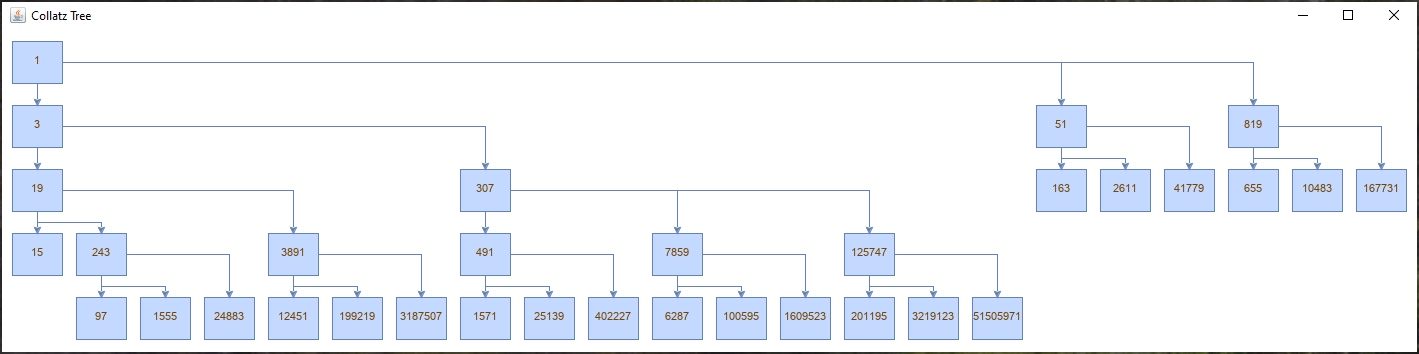
\includegraphics[width=1.00\textwidth]{figures/h_c5b.png}
	\caption{Section of the graph $H_{C,5}$ starting at its root (without branches that reflect a subsequence containing the trivial cycle)}
	\label{fig:4}
\end{figure}

Figure~\ref{fig:4} illustrates a small section of $H_{C,5}$ starting at its root. The particularly interesting thing about the graph $H_{C,5}$ is that it contains three cycles, the trivial cycle starting from the root $1,3$ and two non-trivial cycles $43,17,27$ and $83,33,13$. To be precise, three cycles are known (as it will become apparent later in section~\ref{sec:non_trivial_cycles}), and on the basis of present knowledge it cannot be ruled out with any certainty that other cycles exist.
